\documentclass{beamer}

%%% set Beamer opts %%%

\mode<presentation>
{
  \usetheme{Madrid}       
  \usecolortheme{beaver} 
  \setbeamertemplate{caption}[numbered]
  \setbeamercovered{transparent}
  \setbeamertemplate{itemize items}[default]
  \setbeamertemplate{enumerate items}[default]
  \setbeamercolor{block title}{use=structure,fg=white,bg=red!75!black}
  \setbeamercolor{block body}{use=structure,fg=black,bg=white!20!white}
}


%%% for loop %%%
\usepackage{pgffor}

%%% blind text %%%
\usepackage[english]{babel}
\usepackage{blindtext}

%%% referencing %%%
\usepackage{natbib}
\bibliographystyle{agsm}
\usepackage{amssymb}


%%% figures %%%
\usepackage{subcaption}
\usepackage{graphicx}

%%% animate! %%%
\usepackage{animate}
\usepackage{xmpmulti}

%%% col %%%
\usepackage{xcolor}
\usepackage{listings}

%%% equations %%%
\usepackage{amsmath}
\usepackage{mathabx}
\usepackage{amsfonts}
\usepackage{mathrsfs}
\usepackage{stackengine}


%% algorithms %%
%%% algorithms %%% 
\RequirePackage[lined, ruled]{algorithm2e}


\title[CSM 2021]{Robust Inference for Change Points in Piecewise Polynomials of General Degrees}

\author[]{Shakeel Gavioli-Akilagun \and Piotr Fryzlewicz}

\institute[LSE department of Statistics]{\scshape{London School of Economics \\ Department of Statistics}}

\date[December 2021]{}

\logo{
  \includegraphics[height=3cm]{"../plots/LSE-logo"}
}

\begin{document}


\begin{frame}
  \titlepage
\end{frame}

\logo{}

\section{Inference for Change Points}

\begin{frame}
\tableofcontents[currentsection]
\end{frame}

\begin{frame}{Problem Statement}
We observe data $\mathbf{y_{1:n}} = \left ( y_1, \dots, y_n \right )'$ generated by the following `signal + noise' model

\begin{equation*}
	y_t = f_t^\circ + \zeta_t, \hspace{0.5cm} t = 1, \dots, n
\end{equation*}

\hfill

\begin{itemize}
\item $\zeta$'s sign symmetric and independent, otherwise arbitrary
\item $f^\circ$ piecewise polynomial with known fixed degree
\item \textbf{Goal} inferential statements about unknown change point locations
\end{itemize}
\end{frame}

\begin{frame}{Our Method: piecewise-constant signal}

\only<1>{
\begin{figure}
\centering
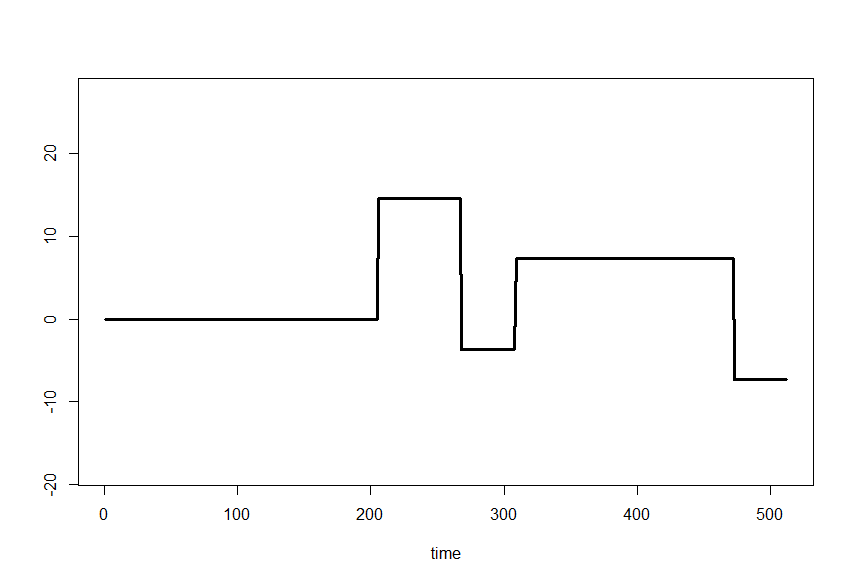
\includegraphics[width=0.75\textwidth]{../plots/bolcks-signal}
\caption{first 512 values of the \texttt{blocks} signal}
\end{figure}
}

\only<2>{
\begin{figure}
\centering
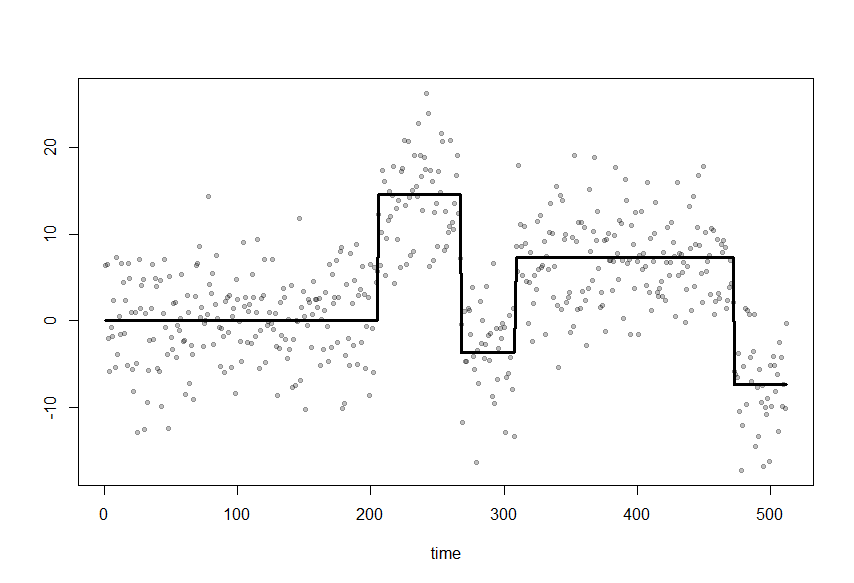
\includegraphics[width=0.75\textwidth]{../plots/bolcks-signal-noise}
\caption{first 512 values of the \texttt{blocks} signal with additive noise}
\end{figure}
}

\only<3>{
\begin{figure}
\centering
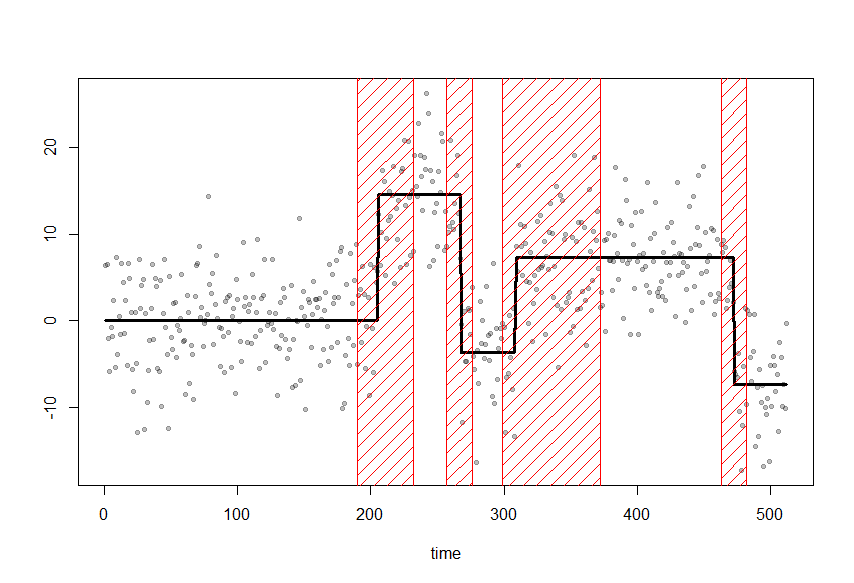
\includegraphics[width=0.75\textwidth]{../plots/bolcks-signal-noise-rects}
\caption{intervals of significance returned by our procedure}
\end{figure}
}
\end{frame}


\begin{frame}{Our Method: piecewise-linear signal}

\only<1>{
\begin{figure}
\centering
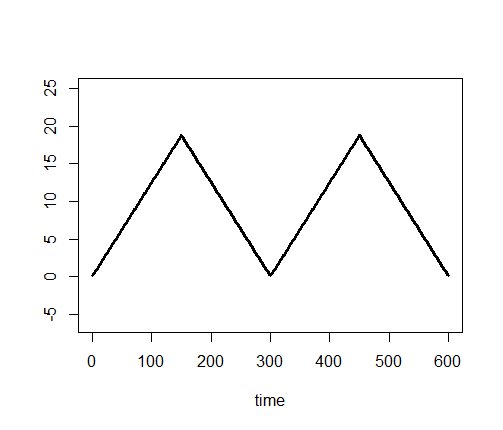
\includegraphics[width=0.65\textwidth]{../plots/waves-signal}
\caption{first 600 values of the \texttt{waves} signal}
\end{figure}
}

\only<2>{
\begin{figure}
\centering
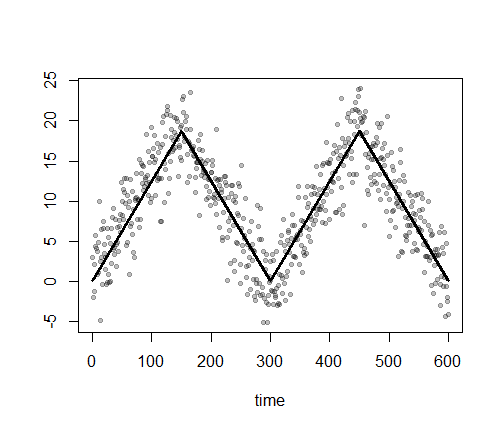
\includegraphics[width=0.65\textwidth]{../plots/waves-signal-noise}
\caption{first 600 values of the \texttt{waves} signal with additive noise}
\end{figure}
}

\only<3>{
\begin{figure}
\centering
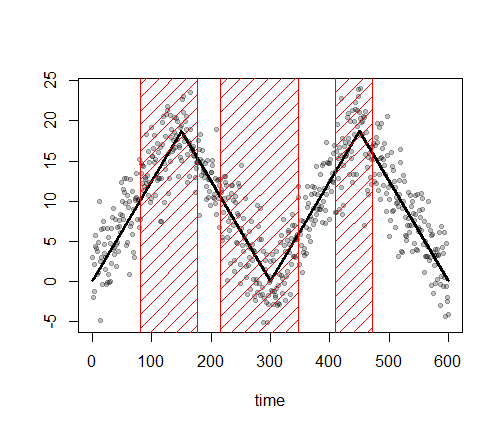
\includegraphics[width=0.65\textwidth]{../plots/waves-signal-noise-rects}
\caption{intervals of significance returned by our procedure}
\end{figure}
}
\end{frame}

\begin{frame}{Background}

\onslide<1>{
\bigskip
Current approaches to change point inference
\begin{itemize}
	\item \textbf{Post selection inference:} \cite{jewell2019testing}, \cite{hyun2021post}, \cite{valiollahi2021change}
	\item \textbf{Simultaneous inference and selection:} \cite{frick2014multiscale}, \cite{pein2015heterogeneous}, \cite{jula2021multiscale}
	\item \textbf{Post inference selection:} \cite{fryzlewicz2020narrowest}, \cite{fryzlewicz2021robust}    
\end{itemize}
}

\onslide<2>{
Our motivations was to...
\begin{itemize}
	\item Generalize \textbf{beyond piecewise constant} signals 
	\item Allow for \textbf{arbitrary error distributions}
	\item Produce a fast - better than $\mathcal{O}(n^2)$ - algorithm
\end{itemize}
}

\end{frame}

\begin{frame}{Recipe for Post Inference Selection \citep{fryzlewicz2020narrowest}}

\begin{enumerate}[<+->]
\item Take a collection of local test $T_{s:e} : \left ( y_s, \dots, y_e \right ) \mapsto \left \{ 0, 1 \right \}$ for
\begin{align*}
	\label{equation: local test}
	& \mathcal{H}_0^{s:e} : \text{  on  } [s,e] \hspace{0.5 cm} f^\circ \in \mathfrak{M} \\
	& \mathcal{H}_1^{s:e} : \text{  on  } [s,e] \hspace{0.5 cm}f^\circ \not\in \mathfrak{M}
\end{align*}


\item Restrict attention to tests with strong false discovery control. For any collection of null sub-intervals $\mathcal{E}$

\begin{equation*}
	\mathbb{P} \left ( \bigcup_{(s,e) \in \mathcal{E}} \left \{ T_{s:e} = 1 \right \} \right ) \leq \alpha
\end{equation*}
\item Apply tests to a sorted grid of sub-intervals; every time a non-null interval is detected explore sub interval for narrowest region of significance then recur to the left / right of detected interval
\end{enumerate}

\end{frame}

%\begin{frame}{Generic Recipe for Post Inference Selection \citep{fryzlewicz2020narrowest}}
%\foreach \nn in {1,2,...,77}{
%\only<\nn>{
%\begin{figure}
%\centering
%\includegraphics[width=0.6\textwidth]{../plots/nsp-illustration/nsp_\nn}
%\end{figure}
%}
%}
%%\end{frame}

\begin{frame}{New Generic Recipe for Inference on Piecewise Polynomials}

\begin{enumerate}[<+->]
\item Given a candidate $f$ define $\hat{\zeta}_t^f = y_t - f_t$; introduce a second local test for whether empirical residuals ``look like noise'' at some level $\alpha$

\begin{equation*}
	\psi_{s:e}^{f,\alpha} : \left ( \hat{\zeta}_s^f, \dots, \hat{\zeta}_e^f \right ) \mapsto \left \{ 0, 1 \right \}
\end{equation*}

\item Then a local $(1-\alpha)$ level confidence set for $f^\circ$ can be obtained by inverting $\psi$ on any sub-interval as follows

\begin{equation*}
	\mathcal{C} \left ( y_{s:e}, \alpha \right ) = \left \{ f: \psi^{f,\alpha}_{s:e} \neq 1 \right \}
\end{equation*}

\item Finally, construct a local test by intersecting the confidence set with polynomials of degree $p$

\begin{equation*}
	T_{s:e} = \mathbf{1} \left \{ \mathcal{C} \left ( y_{s:e}, \alpha \right ) \cap \texttt{poly} (p) \neq \emptyset \right \}
\end{equation*}
\end{enumerate}
\end{frame}

\section{Inference using Runs}

\begin{frame}
\tableofcontents[currentsection]
\end{frame}

\begin{frame}{The Runs Test for Pure Noise}

\begin{exampleblock}{}
We may use the maximum run of the empirical residuals on a sub-interval to decide whether $f$ represents a good local fit

\begin{equation*}
	\psi_{s:e}^f = \mathbf{1} \left \{ \text{max\_run} (\mathbf{y_{s:e} - f_{s:e}}) > \lambda \right \}
	\label{equation: local runs test}
\end{equation*}
\end{exampleblock}

\bigskip

*The maximum run of either sign is given by

\bigskip 

\only<1>{
\texttt{0.24 -0.73  0.79 -1.57 -0.25  -1.36  0.60  0.92 0.00 1.13  0.17}
}

\only<2>{
\texttt{\textcolor{blue}{0.24} \textcolor{red}{-0.73} \textcolor{blue}{0.79} \textcolor{red}{-1.57 -0.25 -1.36}  \textcolor{blue}{0.60  0.92 0.00 1.13  0.17}}
}

\only<3>{
\begin{equation*}
\max \left \{ \omega \in \mathbb{N} : \omega = \left ( \max_{\substack{s \leq j \leq k \leq e \\ k-j+1 = \omega}} \sum_{i=j}^k \mathbf{1}_{\left \{ \hat{\zeta}_i^f \geq 0 \right \}} \bigwedge \max_{\substack{s \leq j \leq k \leq e \\ k-j+1 = M}} \sum_{i=j}^k \mathbf{1}_{\left \{ \hat{\zeta}_i^f < 0 \right \}} \right ) \right \}
\end{equation*}
}

\end{frame}

\begin{frame}{Inverting the Runs Test}

\begin{itemize}[<+->]
\item No need compute the entire confidence set! Enough to compute the point-wise upper and lower bounds then check if a polynomial of the desired degree may pass between them

\begin{align*}
	& l_t = \inf \left \{ f_t : f \in C \left ( \mathbf{y_{s:e}} , \alpha \right ) \right \} \\
	& u_t = \sup \left \{ f_t : f \in C \left ( \mathbf{y_{s:e}} , \alpha \right ) \right \}
\end{align*}

\item From \textbf{\cite{davies1995data}, \cite{davies2001local}} we have that

\begin{align*}
	& u_t = \left\{\begin{matrix}
\min \left \{ u_{t-1}, \max \left \{ y_i : t-\lambda \leq i \leq t \right \}  \right \} & f^\circ \text{  non-increasing}\\
\min \left \{ u_{t+1}, \max \left \{ y_i : t \leq i \leq t + \lambda \right \} \right \} & f^\circ \text{  non-decreasing}
\end{matrix}\right. \\
	& l_t = \left\{\begin{matrix}
\max \left \{ l_{t+1}, \min \left \{ y_i : t \leq i \leq t + \lambda \right \} \right \} & f^\circ \text{  non-increasing} \\
\max \left \{ l_{t-1}, \min \left \{ y_i : t - \lambda \leq i \leq t \right \} \right \} & f^\circ \text{  non-decreasing}
\end{matrix}\right.
\end{align*} \\
\end{itemize}

\end{frame}

\begin{frame}{Practical Testing in the Piecewise Constant Setting}

Data locally agrees with $f^\circ$ being a degree zero polynomial if

\begin{exampleblock}{}
\begin{equation*}
	\min_{s \leq t \leq e} u_t > \max_{s \leq t \leq e} l_t
\end{equation*}
\end{exampleblock}

Can be tested in $\mathcal{O}(1)$ time

\only<1>{
\begin{figure}
\centering
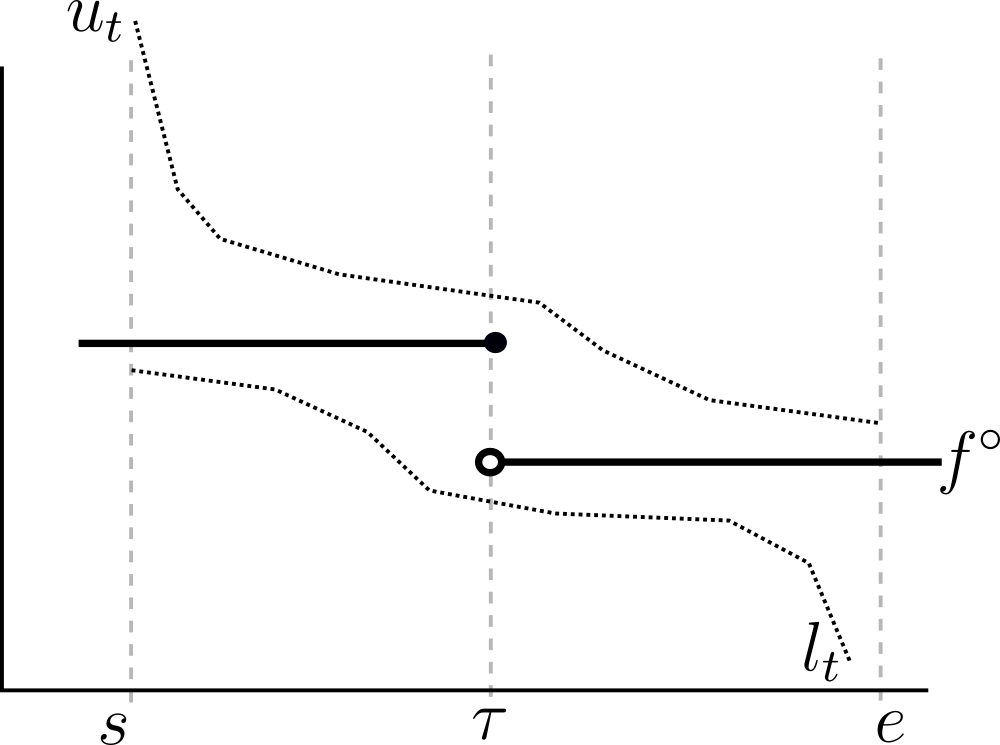
\includegraphics[width=0.45\textwidth]{../plots/pcws-const-detection-1}
\end{figure}
}

\only<2>{
\begin{figure}
\centering
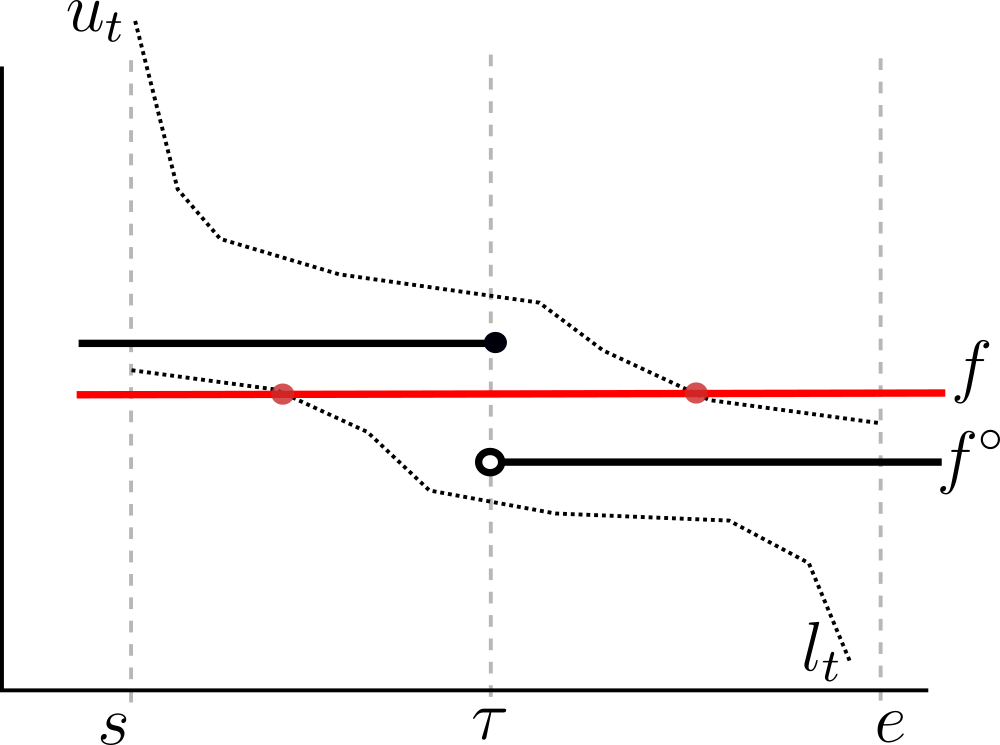
\includegraphics[width=0.45\textwidth]{../plots/pcws-const-detection-2}
\end{figure}
}

\end{frame}


\begin{frame}{Practical Testing in the Piecewise Linear Setting}
Data locally agrees with $f^\circ$ being a polynomial of degree one if

\begin{exampleblock}{}
\begin{equation*}
	\texttt{Hull} \left \{ (s, u_s), \dots, (e, u_e) \right \} \cap \texttt{Hull}  \left \{ (s, l_s), \dots, (e, l_e) \right \} = \emptyset
\end{equation*}
\end{exampleblock}

Can be tested in $\mathcal{O} \left ( \log n \right )$ time \citep{chazelle1987intersection}

\only<1>{
\begin{figure}
\centering

\includegraphics[width=0.45\textwidth]{../plots/pcws-lin-detection-1}
\end{figure}
}

\only<2>{
\begin{figure}
\centering
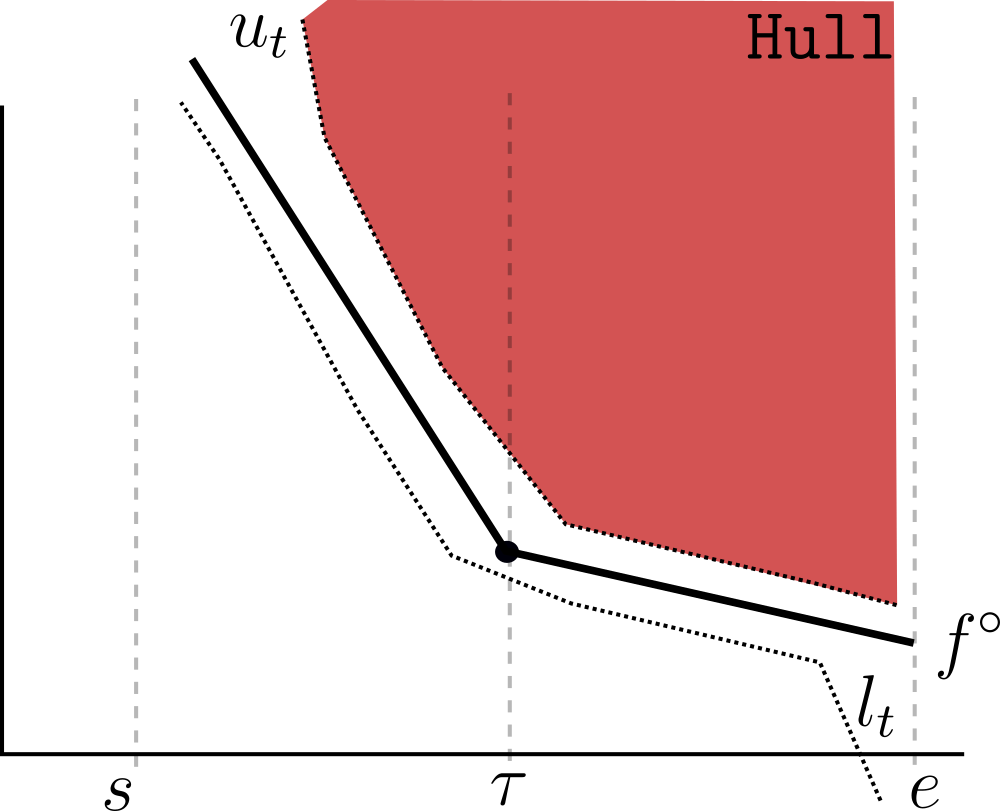
\includegraphics[width=0.45\textwidth]{../plots/pcws-lin-detection-2}
\end{figure}
}

\only<3>{
\begin{figure}
\centering
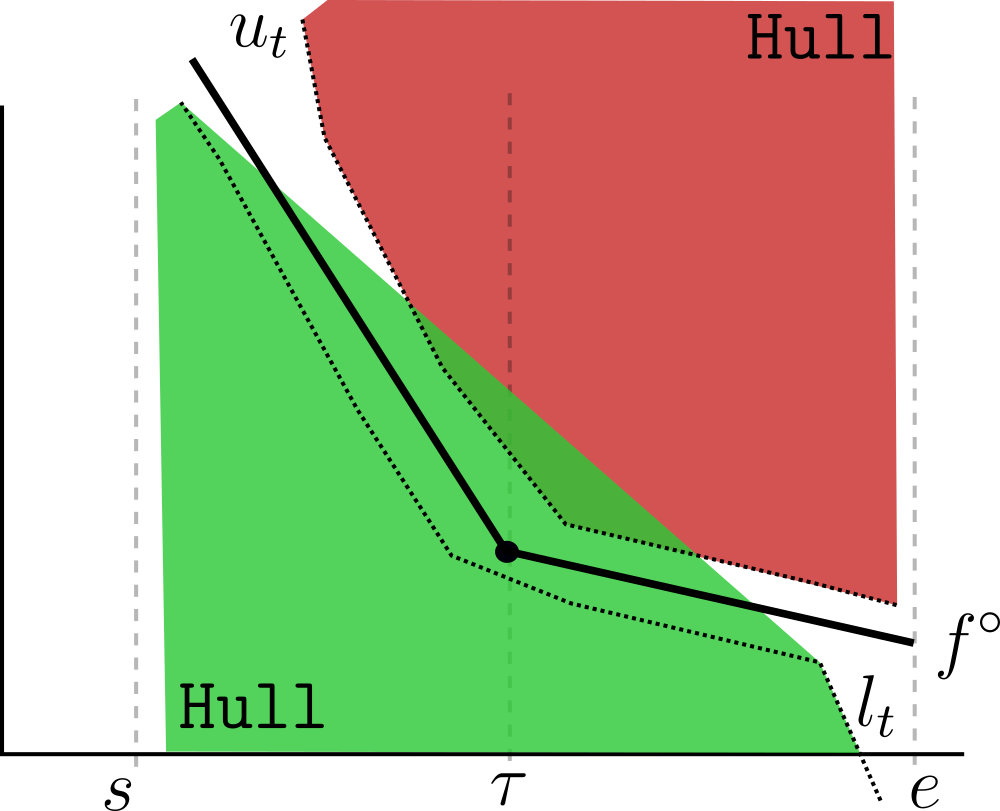
\includegraphics[width=0.45\textwidth]{../plots/pcws-lin-detection-3}
\end{figure}
}

\end{frame}


\section{Theoretical Results}

\begin{frame}
\tableofcontents[currentsection]
\end{frame}

\begin{frame}{Generic Piecewise Polynomial Setting}

\begin{exampleblock}{}
Let $f_{0}, \dots, f_{N}$ be polynomials in $t$ of fixed and known degrees and with  $f_{j} \neq f_{j-1}$. Let $\Theta = \left ( \tau_1, \dots, \tau_N \right ) $ be the set of change point locations, then the signal component is

\begin{equation*}
	f_t^\circ = \sum_{j = 0}^{N} f_{t,j}^\circ \mathbf{1}_{\left \{ t \in [\tau_{j-1}, \tau_j) \right \}}
\end{equation*}
\end{exampleblock}
\bigskip

\textbf{(A1)}  $\mathbb{P} \left ( \zeta_t > 0 \right ) = \mathbb{P} \left ( \zeta_t \leq 0 \right ) = \frac{1}{2}$ for all $t = 1, 2, \dots$

\bigskip 

\textbf{(A2)} $\mathbb{P} \left ( \zeta_t > 0 \mid \zeta_s \right ) = \mathbb{P} \left ( \zeta_t > 0 \right )$ for all $t \neq s$

\end{frame}

\begin{frame}{Exact Coverage Guarantees}
\begin{alertblock}{}
Let A1 - A2 hold and $\left \{ \hat{I}, \dots, \hat{I}_{\hat{N}} \right \}$ be the set of intervals returned by our algorithm in any generic piecewise polynomial setting with a threshold $\lambda = \lambda_n$ chosen as shown below 
\begin{equation*}
	\lambda_n = \log_2 \left ( n - 1 \right ) + \log_2 \left ( \frac{1}{\log \left ( \frac{1}{1-\alpha} \right )} \right )
	\label{equation: naive threshold}
\end{equation*}

Then the following guarantee holds

\begin{equation*}
	\mathbb{P} \left ( \bigcup_{j=1}^{\hat{N}} \left \{ \hat{I}_j \cap \Theta = \emptyset \right \} \right ) \leq \alpha + \frac{0.3}{n-2}
\end{equation*}
\end{alertblock}
\end{frame}


\begin{frame}{The Piecewise Constant Setting}

\begin{exampleblock}{}
For some constants $\theta_0, \dots, \theta_{N}$ with $\theta_j \neq \theta_{j-1}$ the signal component is
\begin{equation*}
	f_t^\circ = \sum_{j = 0}^{N} \theta_j \mathbf{1}_{\left \{ t \in [\tau_{j-1}, \tau_j) \right \}}
\end{equation*}
\end{exampleblock}

\bigskip

\textbf{(A3)} Minimum change point spacing is of the order $\mathcal{O}(n)$ \\ 

\bigskip

\textbf{(A4)} There is a random variable $\xi$ such that $\mathbb{P} \left ( |\zeta_t| > x \right ) \leq \mathbb{P} \left ( |\xi| > x \right )$ for any $x>0$ and for all $t=1,2,\dots$ \\ 

\bigskip

\textbf{(A5)} $\exists \beta \in (0, \frac{1}{2})$ such that if $x \in [0,1]$ then $\mathbb{P} \left ( |\xi| > x \right ) \leq \frac{1}{2} - \beta x$

\end{frame}


\begin{frame}{Interval Sub-Sampling \citep{fryzlewicz2020narrowest}}

\bigskip 

\begin{enumerate}[<+->]
\item Chooses an integer $M$ which determines how many local test may be applied. Define an integer 

\begin{equation*}
	k^* = \left \lfloor \left ( 1+\sqrt{1+8M} \right ) / 2 \right \rfloor
\end{equation*}

\item Define a shift term

\begin{equation*}
	\delta_M = \left \lfloor \frac{n-1}{k^*-1} \right \rfloor
\end{equation*}

\item Draw all sub-intervals in $\left \{ 1, \dots, k^* \right \}$ and re-map to $\left \{ 1, \dots, n \right \}$ according to the rule

\begin{equation*}
\left (s, e \right ) \mapsto \left ( \left (s-1 \right )\times \delta_M + 1, \left (e-1 \right )\times \delta_M + 1 \right )
\end{equation*}
\end{enumerate}


\end{frame}


\begin{frame}{Change Point Detection Guarantees}

\begin{alertblock}{}
Grant assumption A1 - A5 and let $\left \{ \hat{I}_1, \dots, \hat{I}_{\hat{N}} \right \}$ be the intervals returned by our algorithm in the piecewise constant setting. Define

\begin{equation*}
	\mathcal{A}_n = \left \{ \hat{N} = N, \forall j = 1, \dots, N \hspace{0.1cm} \exists k \hspace{0.1cm} \text{s.t.} \left \{ \hat{I}_j \cap \Theta \right \} = \tau_k \right \} 
\end{equation*}

If the number of local tests is chosen as $M = M_n$ such that $M_n \rightarrow \infty$ as n diverges then writing $\Delta = \min_j \left | \theta_j - \theta_{j-1} \right |$ the following guarantee holds

\begin{equation*}
	\mathbb{P} \left ( \mathcal{A}_n \right ) \geq 1 - \left ( \alpha + \frac{0.3}{n-2} + C_N \exp \left ( - C_{M,\beta, \alpha} \times n^{1-\log_2 \left ( \frac{2}{1+\beta \Delta} \right ) } \right ) \right )
\end{equation*}
\end{alertblock}

\onslide<2>{
\begin{alertblock}{}
w.p.a.-$(1-\alpha)$ our algorithm detects all change points and isolates them to their own interval as long as the minimum jump size satisfies
\begin{equation*}
	\Delta > \left (\beta \log_2 n \right ) ^ {-1}
\end{equation*}
\end{alertblock} 
}
\end{frame}

\section{Numerical Illustration}

\begin{frame}
\tableofcontents[currentsection]
\end{frame}


\begin{frame}{Alternative Approaches from the Literature}

\begin{itemize}
	\item \textbf{\cite{fryzlewicz2021robust}} [MR] obtains  simultaneous confidence intervals for $\Theta = \left  ( \tau_1, \dots, \tau_N \right )$ using local tests based

\begin{equation*}
	T_{s:e} = \mathbf{1} \left \{ \min_{f \in \mathbb{R}} \left \| \text{sgn}(y_{s:e} - f \boldsymbol{1}_{s:e}) \right \|_{MR} > \lambda \right \} 
\end{equation*}	

\bigskip

	\item \textbf{\cite{jula2021multiscale}} [MQS] produces a confidence set for $f^\circ$ by inverting local tests
	
\begin{equation*}
\psi_{s:e}^f = \mathbf{1} \left \{ \sqrt{2 \mathcal{L} \left ( y_{s:e}, f \right )} - \sqrt{2 \log \left ( \frac{e n}{e-s+1} \right )} > q_n \left ( \alpha \right ) \right \}
\end{equation*}
\end{itemize}

\end{frame}

\begin{frame}{Execution Speed}

\only<1>{
\begin{figure}
\centering
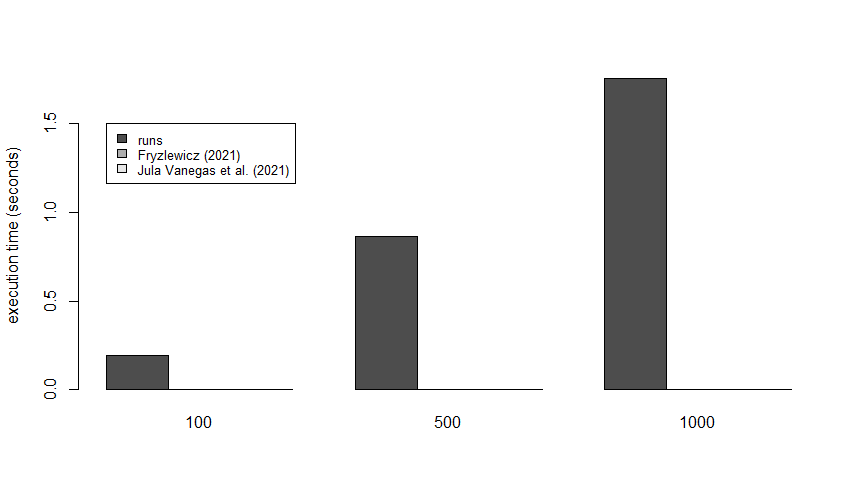
\includegraphics[width=0.75\textwidth]{../plots/execution-times-1}
\caption{execution times on Gaussian noise, using 2.59 GHz Intel Core i7 CPU}
\end{figure}
}

\only<2>{
\begin{figure}
\centering
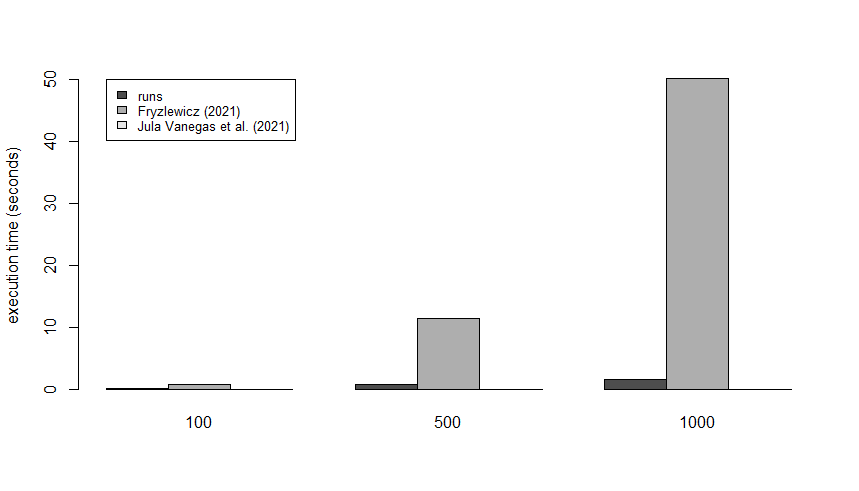
\includegraphics[width=0.75\textwidth]{../plots/execution-times-2}
\caption{execution times on Gaussian noise, using 2.59 GHz Intel Core i7 CPU}
\end{figure}
}

\only<3>{
\begin{figure}
\centering
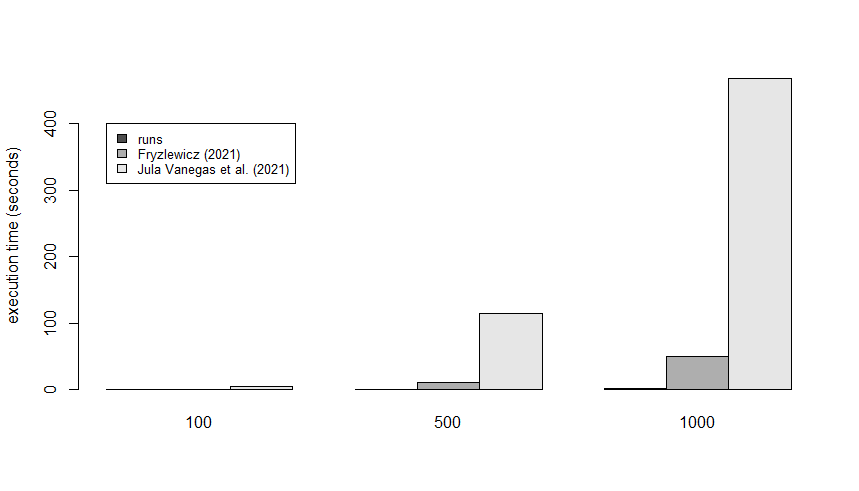
\includegraphics[width=0.75\textwidth]{../plots/execution-times-3}
\caption{execution times on Gaussian noise, using 2.59 GHz Intel Core i7 CPU}
\end{figure}
}

\only<4>{
\begin{figure}
\centering
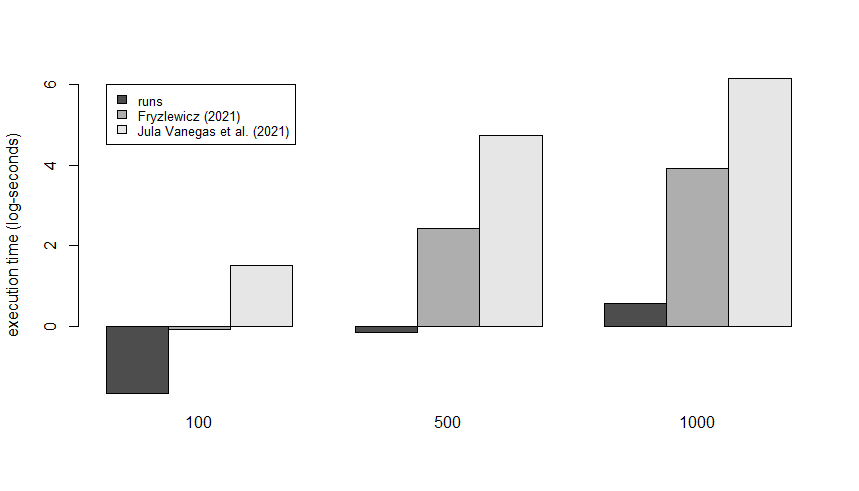
\includegraphics[width=0.75\textwidth]{../plots/execution-times-4}
\caption{execution times on Gaussian noise, using 2.59 GHz Intel Core i7 CPU}
\end{figure}
}

\end{frame}

\begin{frame}{Coverage Guarantees: pure noise test-beds}

\begin{figure}
\centering
\begin{subfigure}[b]{0.3\textwidth}
    \centering
    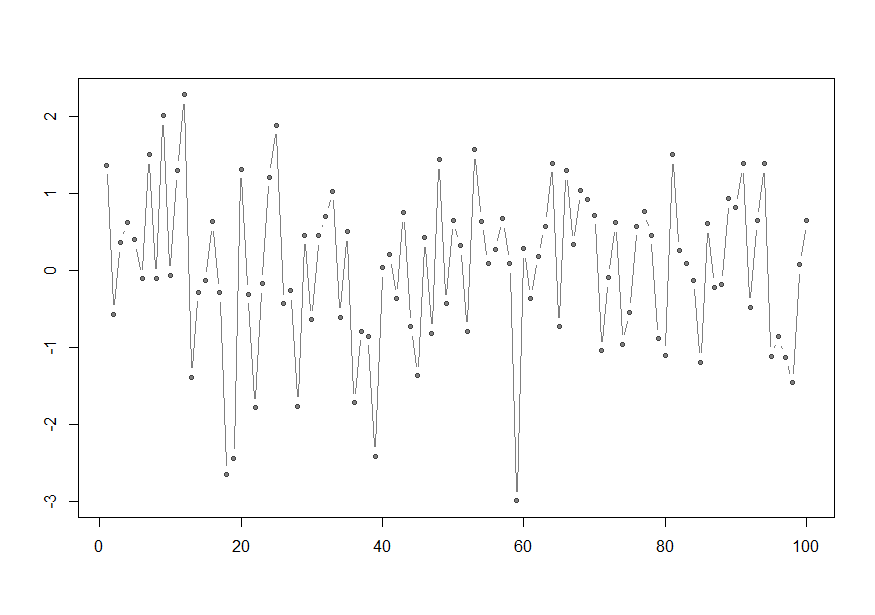
\includegraphics[width=\textwidth]{../plots/plain-gauss}
    \caption{Gaussian}
\end{subfigure}
\begin{subfigure}[b]{0.3\textwidth}
    \centering
    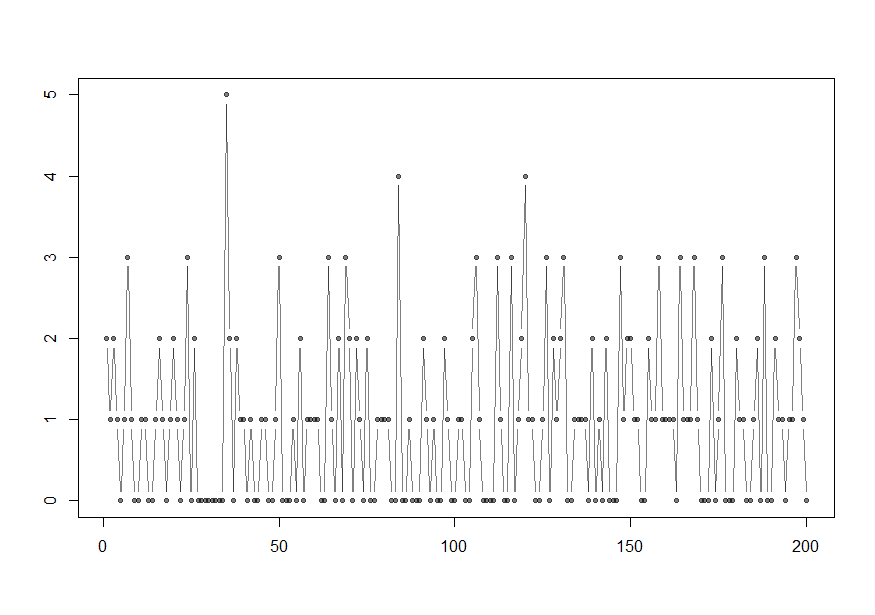
\includegraphics[width=\textwidth]{../plots/plain-poisson}
    \caption{Poisson}
\end{subfigure}
\begin{subfigure}[b]{0.3\textwidth}
    \centering
    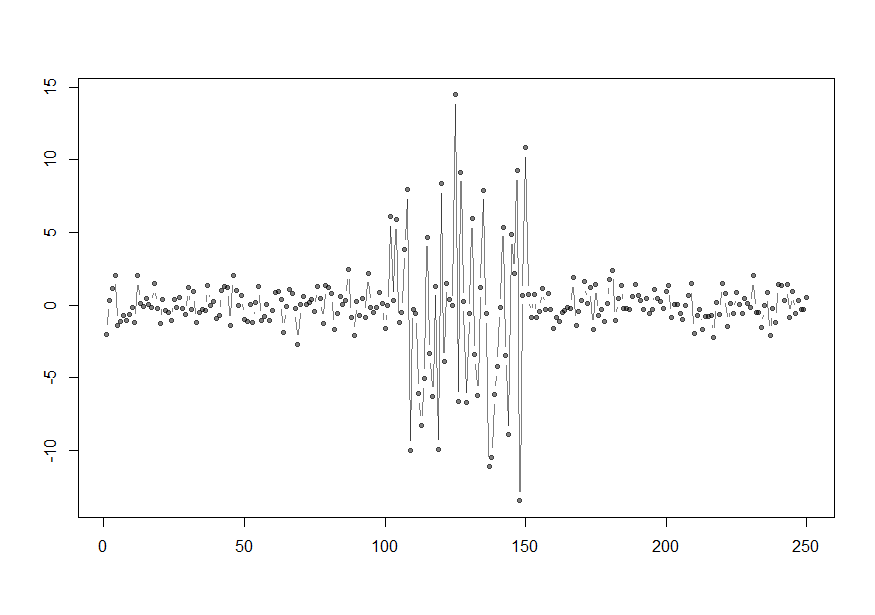
\includegraphics[width=\textwidth]{../plots/hetero-gauss}
    \caption{Gaussian (hetero)}
\end{subfigure}
\begin{subfigure}[b]{0.3\textwidth}
    \centering
    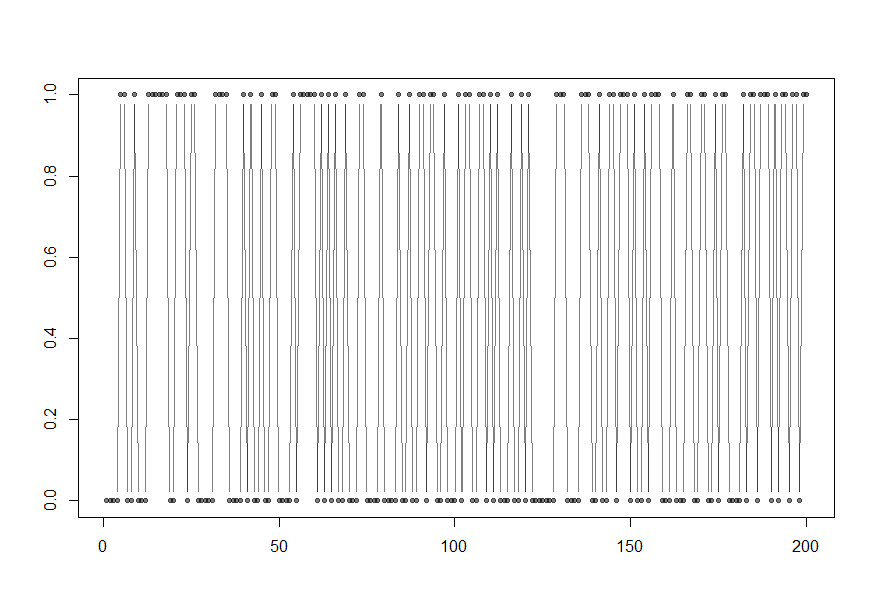
\includegraphics[width=\textwidth]{../plots/sym-bern}
    \caption{Symmetric Bernoulli}
\end{subfigure}
\begin{subfigure}[b]{0.3\textwidth}
    \centering
    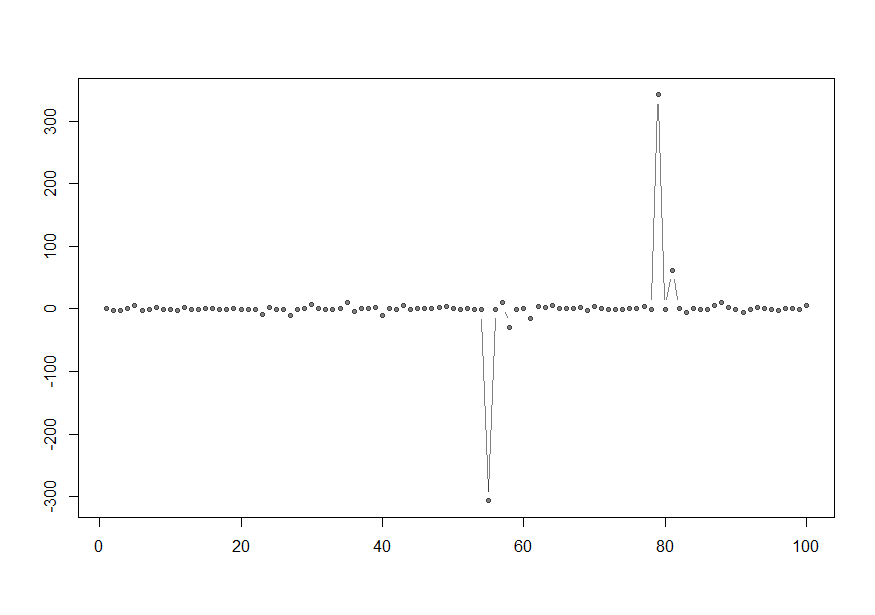
\includegraphics[width=\textwidth]{../plots/plain-cauchy}
    \caption{Cauchy}
\end{subfigure}
\begin{subfigure}[b]{0.3\textwidth}
    \centering
    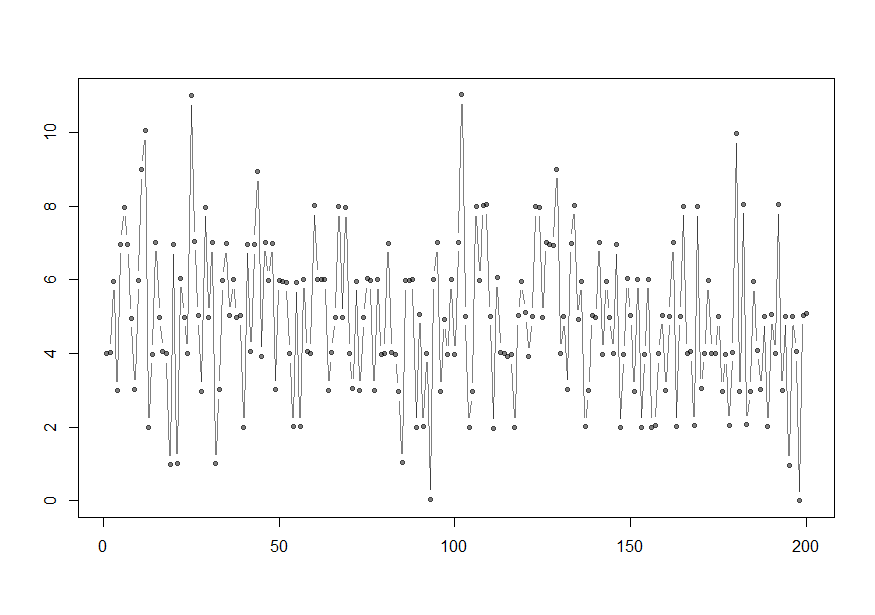
\includegraphics[width=\textwidth]{../plots/poisson-normal-mix}
    \caption{Poisson + Gaussian}
\end{subfigure}
\end{figure}

\end{frame}


\begin{frame}{Coverage Guarantees: simulation results}

Number of times, out of 100 simulated sample paths, that a particular method indicates no intervals of significance:

\bigskip

\centering
\resizebox{0.65\textwidth}{!}{%
\begin{tabular}{@{\extracolsep{5pt}} lccc} 
\\[-1.8ex]\hline 
\hline \\[-1.8ex] 
 & runs & MR & MQS \\ 
\hline \\[-1.8ex] 
Plain Gauss & $99$ & $100$ & $57$\\ 
Plain Poisson & $100$ & $99$ & $90$\\ 
Heterogeneous Gauss & $100$ & $100$ & $61$\\ 
Symmetric Bernoulli & $99$ & $92$ & $81$\\ 
Plain Cauchy & $99$ & $100$ & $59$\\ 
Mix & $96$ & $100$ & $68$\\ 
\hline \\[-1.8ex] 
\end{tabular}
} 

\end{frame}

\begin{frame}{Detection Power: signal + noise test-beds}
\begin{figure}
\centering
\begin{subfigure}[b]{0.35\textwidth}
    \centering
    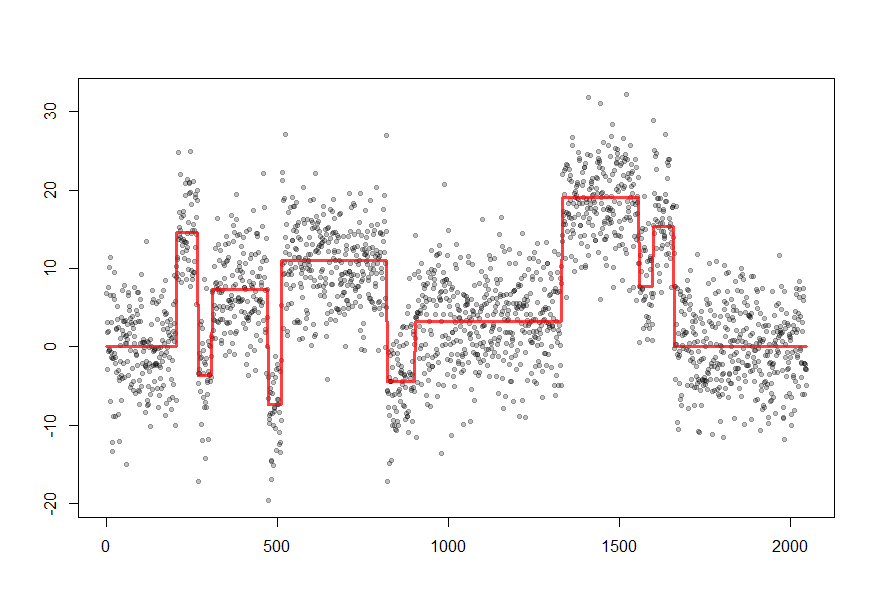
\includegraphics[width=\textwidth]{../plots/blocks-testbed}
    \caption{Blocks}
\end{subfigure}
\begin{subfigure}[b]{0.35\textwidth}
    \centering
    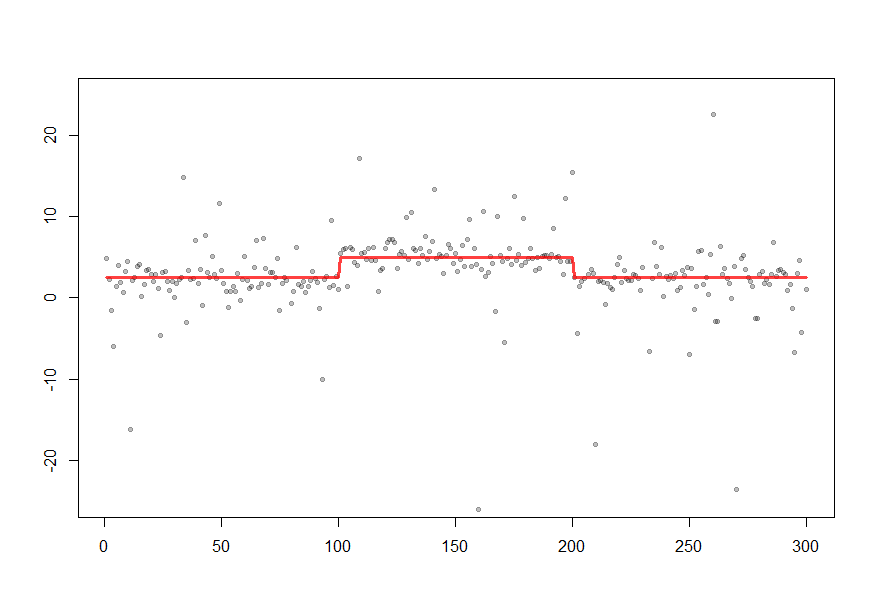
\includegraphics[width=\textwidth]{../plots/cauchy-testbed}
    \caption{Cauchy}
\end{subfigure}
\begin{subfigure}[b]{0.35\textwidth}
    \centering
    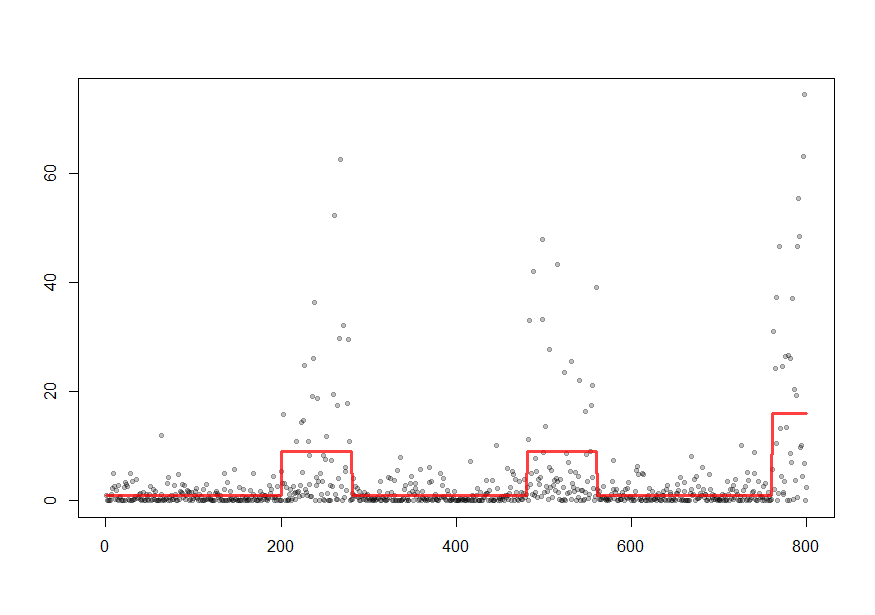
\includegraphics[width=\textwidth]{../plots/bursts-testbed}
    \caption{Bursts}
\end{subfigure}
\begin{subfigure}[b]{0.35\textwidth}
    \centering
    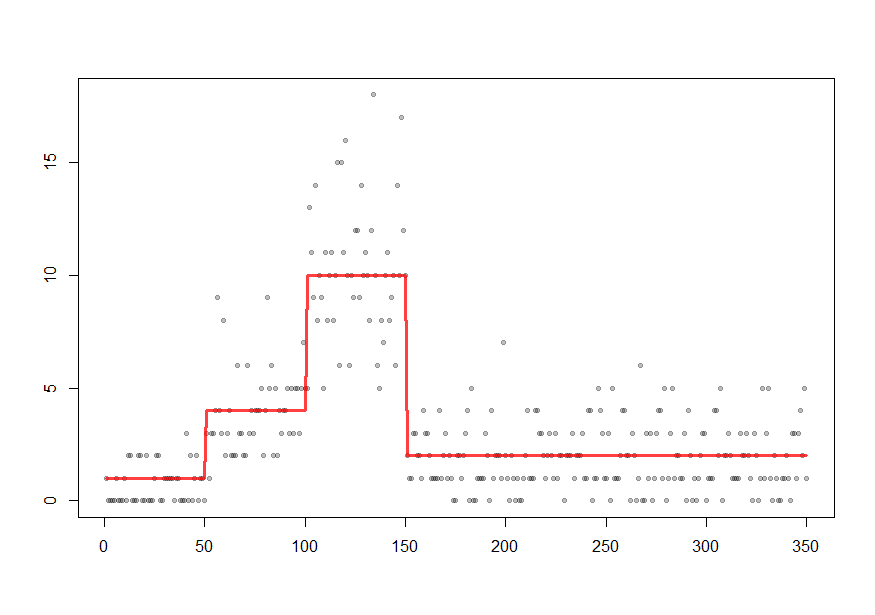
\includegraphics[width=\textwidth]{../plots/poisson-testbed}
    \caption{Poisson}
\end{subfigure}
\end{figure}
\end{frame}


\begin{frame}{Detection Power: simulation results}

Average performance on 100 simulated sample paths of the test beds for each change point inference method: 

\vfill

\centering
\only<1>{
\resizebox{0.75\textwidth}{!}{%
\begin{tabular}{@{\extracolsep{5pt}} lcccccc} 
\\[-1.8ex]\hline 
\hline \\[-1.8ex] 
& \multicolumn{3}{c}{\textbf{Blocks}} & \multicolumn{3}{c}{\textbf{Cauchy}} \\
 & runs & MR & MQS & runs & MR & MQS \\ 
\hline \\ 
Spurious & $0.00$ & $0.00$ & $0.38$ & $0.00$ & $0.00$ & $0.21$ \\
Prop. Genuine & $1.00$ & $1.00$ & $0.96$ & $1.00$ & $1.00$ & $0.91$ \\
No. Genuine & $8.70$ & $9.88$ & $10.79$ & $1.36$ & $2.00$ & $1.96$ \\
Avg. Length & $48.06$ & $46.44$ & $44.86$ & $75.01$ & $60.08$ & $51.90$ \\
\hline   
\end{tabular} 
}
}

\only<2>{
\resizebox{0.75\textwidth}{!}{%
\begin{tabular}{@{\extracolsep{5pt}} lcccccc} 
\\[-1.8ex]\hline 
\hline \\[-1.8ex] 
& \multicolumn{3}{c}{\textbf{Bursts}} & \multicolumn{3}{c}{\textbf{Poisson}} \\
 & runs & MR & MQS & runs & MR & MQS \\ 
\hline \\ 
Spurious & $0.02$ & $0.00$ & $0.13$ & $0.00$ & $0.00$ & $0.07$ \\
Prop. Genuine & $0.99$ & $1.00$ & $0.97$ & $1.00$ & $1.00$ & $0.98$ \\
No. Genuine & $1.25$ & $3.12$ & $4.16$ & $2.27$ & $2.92$ & $2.86$ \\
Avg. Length & $114.29$ & $100.68$ & $114.21$ & $35.80$ & $36.41$ & $31.88$ \\
\hline   
\end{tabular} 
}
}

\end{frame}

\begin{frame}{Real Data Analysis: air quality and COVID lock-downs}

\only<1>{
\begin{figure}
\centering
\begin{subfigure}[b]{0.3\textwidth}
    \centering
    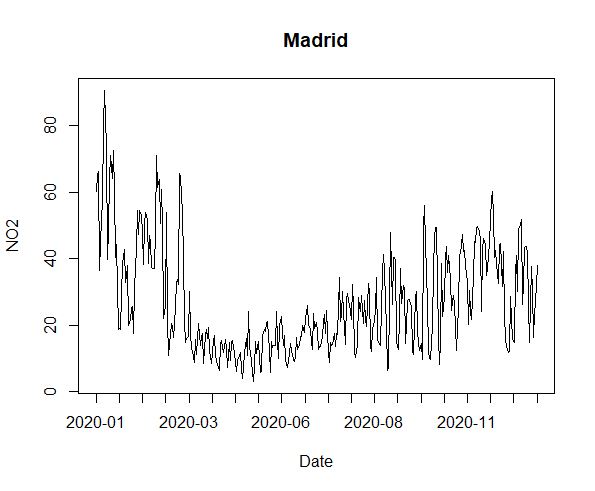
\includegraphics[width=\textwidth]{../plots/Madrid-1}
\end{subfigure}
\begin{subfigure}[b]{0.3\textwidth}
    \centering
    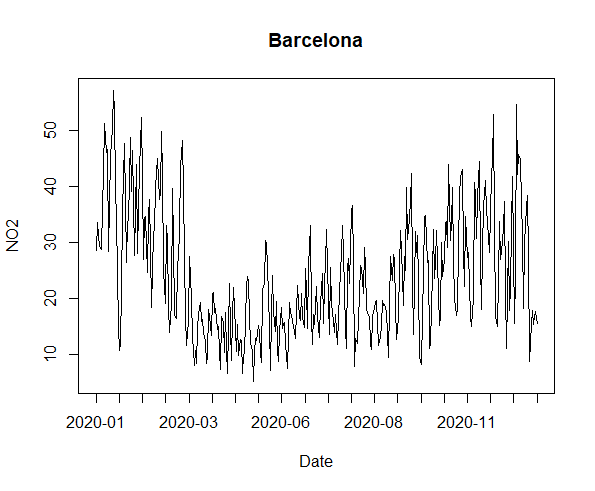
\includegraphics[width=\textwidth]{../plots/Barcelona-1}
\end{subfigure}
\vfill
\begin{subfigure}[b]{0.3\textwidth}
    \centering
    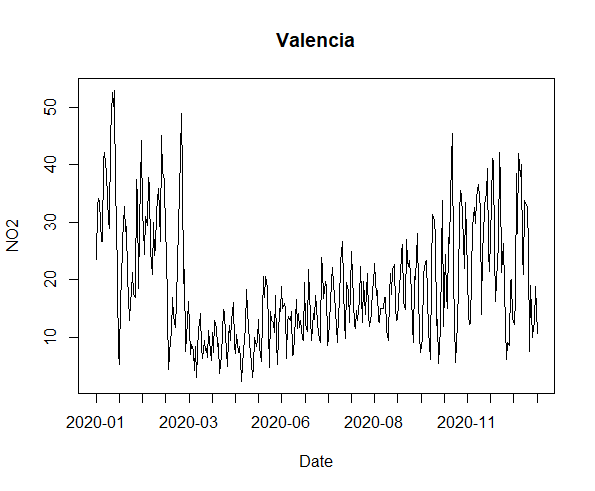
\includegraphics[width=\textwidth]{../plots/Valencia-1}
\end{subfigure}
\begin{subfigure}[b]{0.3\textwidth}
    \centering
    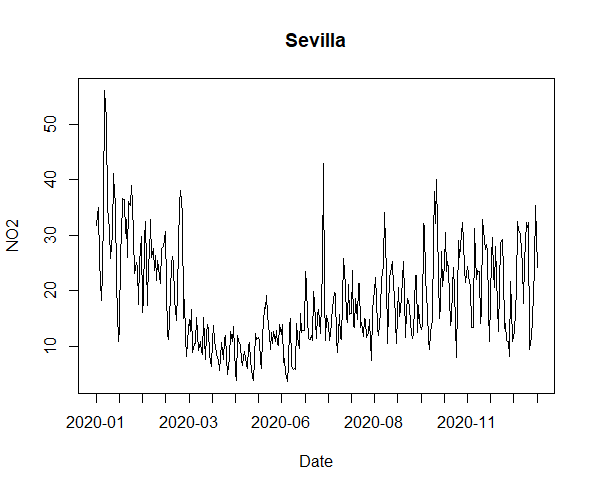
\includegraphics[width=\textwidth]{../plots/Sevilla-1}
\end{subfigure}
\caption{daily $NO_2$ concentration levels during 2020, de-trended and whitened, for the four largest cities in Spain by population}
\end{figure}
}

\only<2>{
\begin{figure}
\centering
\begin{subfigure}[b]{0.3\textwidth}
    \centering
    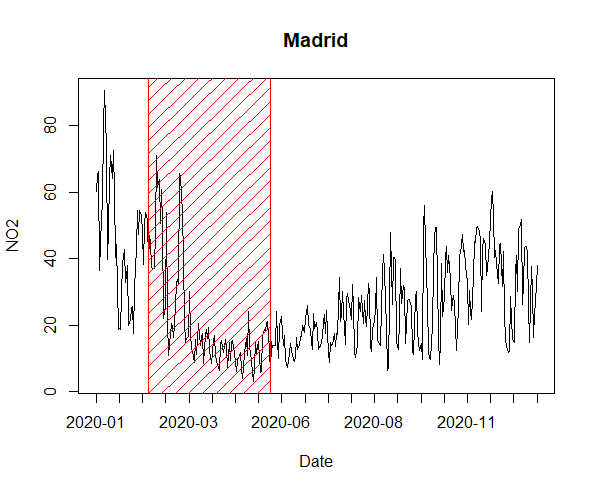
\includegraphics[width=\textwidth]{../plots/Madrid-2}
\end{subfigure}
\begin{subfigure}[b]{0.3\textwidth}
    \centering
    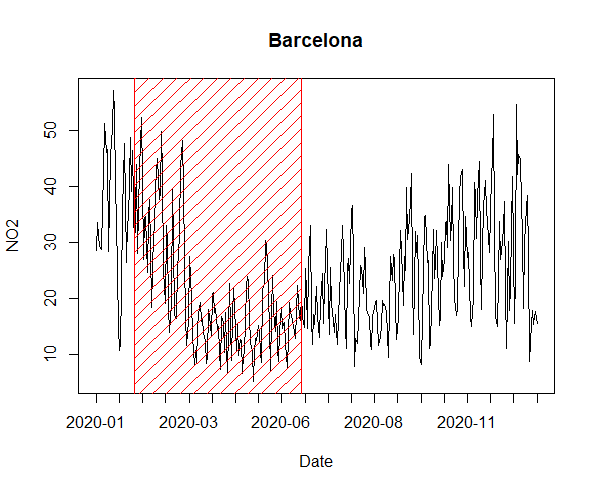
\includegraphics[width=\textwidth]{../plots/Barcelona-2}
\end{subfigure}
\vfill
\begin{subfigure}[b]{0.3\textwidth}
    \centering
    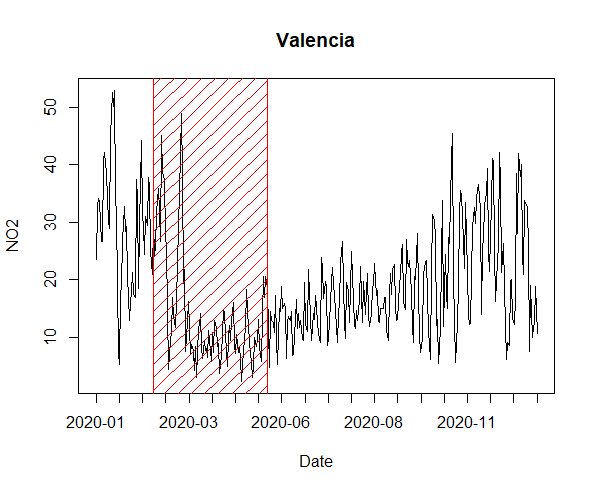
\includegraphics[width=\textwidth]{../plots/Valencia-2}
\end{subfigure}
\begin{subfigure}[b]{0.3\textwidth}
    \centering
    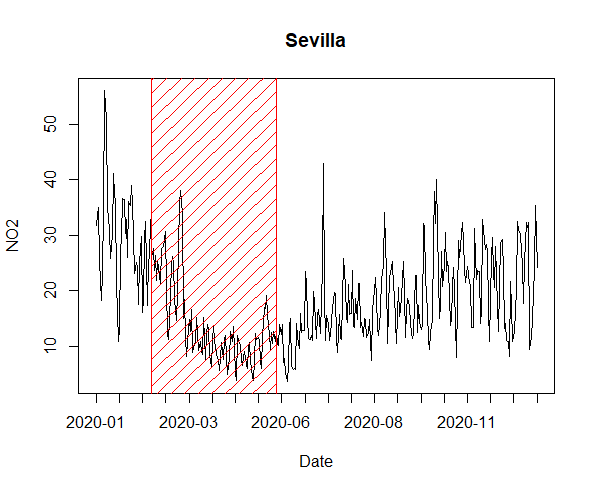
\includegraphics[width=\textwidth]{../plots/Sevilla-2}
\end{subfigure}
\caption{intervals of significance returned by our procedure, testing against $f^\circ$ begin degree 1 polynomial with $\alpha = 0.1$, roughly align with the national state of alarm (March 15) and initial lock-down easing (May 2)}
\end{figure}
}
\end{frame}

\begin{frame}
\centering
\huge{Thank you!}
\end{frame}

\begin{frame}<beamer:0>
    \bibliography{../bibliography/ref}
\end{frame}


\end{document}
